\chapter{مدل‌های نورونی} \label{chap:neuron}

نورون‌ها اجزای زیست‌فیزیکی و زیست‌شیمیایی بسیار پیچیده‌ای هستند.
بنابراین، طراحی و ارائه مدل‌های دینامیکی از نورون نیازمند درکی عمیق از سازوکارهایی است که فعالیت‌های نورونی را تولید و کنترل می‌کنند.
در نتیجه، پیش از طراحی یک مدل لازم است شهودی دقیق نسبت به عوامل مهم در رفتار نورون و آنچه می‌توان نادیده گرفت، به دست آورد.

به همین منظور، در ابتدای این فصل، ساختار نورون را مورد بررسی قرار می‌دهیم.
سپس با بهره‌گیری از این شناخت، مدل‌های مختلفی را برای توصیف رفتار دینامیکی نورون معرفی می‌کنیم.
در نهایت، به بررسی دقیق‌تر نگاشت چیالوو\LTRfootnote{Chialvo map} پرداخته و با رفتار دینامیکی و فضای فاز این مدل آشنا می‌شویم.

\section{نورون}
ساختار نورون را می‌توان به سه بخش اصلی تقسیم کرد:
۱- بدنه سلولی\LTRfootnote{Soma}، واحد پردازش مرکزی نورون که سیگنال‌های ورودی را پردازش می‌کند.
۲- دندریت‌ها\LTRfootnote{Dentrite}، رشته‌هایی درخت مانند که نقش گیرنده‌های ورودی نورون را دارند و سیگنال‌ها را از نورون‌های دیگر جمع‌آوری کرده و به بدنه سلولی منتقل می‌کنند.
۳- آکسون\LTRfootnote{Axon}، بخش خروجی نورون که سیگنال‌های پردازش شده توسط بدنه سلولی را به دیگر نورون‌ها منتقل می‌کند.
هر نورون یک آکسون دارد، اما این آکسون می‌تواند منشعب شده و اطلاعات را به نقاط مختلف مغز ارسال کند.
بسیاری از شاخه‌های آکسون به نورون‌های نزدیک ختم می‌شوند، اما آکسون می‌تواند تا چندین سانتی‌متر کشیده شود تا به نورون‌های دیگر نواحی مغز نیز برسد.
در برخی موارد، آکسون می‌تواند طول کل بدن را طی کند
\cite{dayan2001,gerstner2002,rabinovich2006,trappenberg2022}.
در
\autoref{fig:neuron}
می‌توانید بخش‌های مختلف یک نورون را مشاهده کنید.

\begin{figure}[!ht]
    \centering
    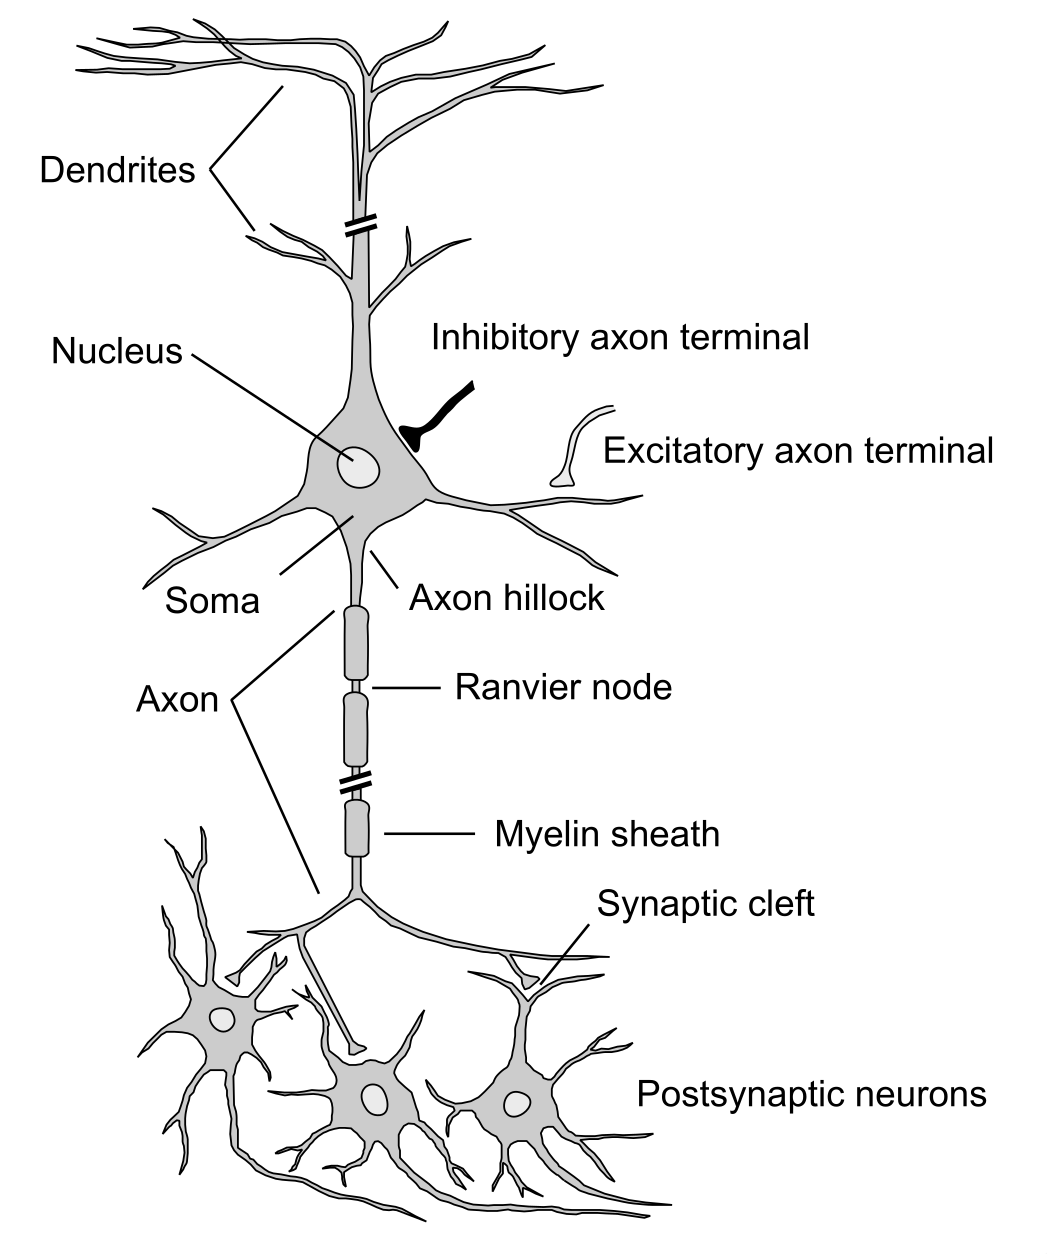
\includegraphics[width=0.6\textwidth]{figures/neuron}
    \caption[ساختار نورون]{ساختار نورون \cite{trappenberg2022}}
    \label{fig:neuron}
\end{figure}

نورون‌ها با تولید پالس‌های الکتریکی مشخصی به نام پتانسیل عمل یا اسپایک، سیگنال‌های الکتریکی را انتقال می‌دهند
\cite{dayan2001}.
پتانسیل عمل، یک تغییر ناگهانی و گذرا در پتانسیل غشای سلولی است.
اگر مجموع ورودی‌ها به یک نورون از یک حد آستانه مشخص فراتر برود، سیگنال خروجی تولید می‌شود.
این سیگنال تولید شده از طریق آکسون به نورون‌های دیگر منتقل می‌شود
\cite{gerstner2002}.
به طور کلی، نورون‌ها به خودی خود پتانسیل عمل شلیک نمی‌کنند بلکه در نتیجه پتانسیل عمل‌های ورودی از نورون‌های دیگر، یک پتانسیل عمل شلیک می‌کنند
\cite{izhikevich2006}.

محل تماس آکسون یک نورون به دندریت (یا بدنه سلولی) نورونی دیگر، سیناپس\LTRfootnote{Synapse} نام دارد.
رایج‌ترین نوع سیناپس در مغز مهره‌داران، سیناپس شیمیایی است.
در یک سیناپس شیمیایی، پایانه آکسون به نورون پس‌سیناپسی\LTRfootnote{Postsynaptic} بسیار نزدیک می‌شود و تنها یک شکاف کوچک بین غشای سلولی نورون پیش‌سیناپسی\LTRfootnote{Presynaptic} و نورون پس‌سیناپسی باقی می‌گذارد که به آن شکاف سیناپسی\LTRfootnote{Synaptic gap} می‌گویند.
به محض اینکه انتقال‌دهنده‌های عصبی به سمت پس‌سیناپسی رسیدند، توسط گیرنده‌های خاصی در غشای سلولی نورون پس‌سیناپسی شناسایی می‌شوند و کانال‌های خاصی را باز می‌کنند تا یون‌های مشخصی به درون یا به بیرون سلول جریان پیدا کنند
\cite{gerstner2002}.
بسته به ماهیت جریان یونی، سیناپس‌ها می‌توانند اثر تحریک‌کننده یا مهاری بر نورون پس‌سیناپسی داشته باشند
\cite{dayan2001}.

نورون‌ها، مانند سایر سلول‌ها، توسط غشایی محصور شده‌اند که فضای داخلی سلول را از فضای خارج آن جدا می‌کند.
غشای سلولی از دو لایه‌ی نازک لیپیدی به ضخامت ۳ تا ۴ نانومتر تشکیل شده که اساساً یک عایق الکتریکی تقریباً کامل بوده و برای اکثر یون‌ها غیرقابل نفوذ است
\cite{gerstner2002}.
عایق بودن غشاء منجر به جدا شدن بارهای الکتریکی موجود در سطح داخلی و خارجی آن می‌شود.
این جدا شدن بار‌های الکتریکی باعث می‌شود غشاء به شکل یک خازن عمل کند
\cite{dayan2001}.

با این حال، پروتئین‌های خاصی در غشای سلولی وجود دارند که به عنوان دریچه‌های برای عبور یون‌ها عمل کرده و باعث می‌شوند بارهای الکتریکی بتوانند از غشاء عبور کنند
\cite{gerstner2002}.
غنای دینامیکی و پیچیدگی محاسباتی نورون‌ها به دلیل وجود همین پروتئین‌ها در غشای سلولی است
\cite{graben2008}.
دو نوع دریچه یونی در غشای سلولی وجود دارد؛
پمپ‌های یونی و کانال‌های یونی.
بسیاری از این کانال‌ها، اما نه همه، شدیداً انتخابی هستند و تنها به یک نوع یون اجازه عبور می‌دهند
\cite{dayan2001}.
در حالی که کانال‌های یونی مانند یک حفره در غشاء عمل کرده و اجازه می‌دهند یون‌ها از چگالی بیشتر به چگالی کمتر بروند.
پمپ‌های یونی به طور فعال یون‌ها را از سمتی که چگالی کمتری دارند به سمتی که چگالی بیشتر دارند، منتقل می‌کنند.
در نتیجه، غلظت یون در مایع درون سلولی با غلظت یون‌های اطراف سلول متفاوت است.

بعضی از این کانال‌ها منافذی همیشه باز دارند و تنها به یون‌هایی مانند سدیم
(\ce{Na+})،
پتاسیم
(\ce{K+})،
کلسیم
(\ce{Ca^2+})
و کلراید
(\ce{Cl-})
اجازه عبور می‌دهند.
به همین دلیل به این کانال‌ها، کانال‌های نشتی می‌گویند.
این کانال‌های یونی همیشه باز، پتانسیل استراحت نورون‌ها را کنترل می‌کنند
\cite{trappenberg2022}.
کانال‌های دیگری نیز وجود دارند که توسط پتانسیل غشاء یا حضور برخی مواد خاص در اطراف نورون کنترل می‌شوند
\cite{graben2008}.
کانال‌های یونی با باز و بسته شدن در واکنش به تغییر پتانسیل و سیگنال‌های ورودی و خروجی، جریان یون‌ها را در سراسر غشای سلولی کنترل می‌کنند
\cite{dayan2001}.

\begin{figure}[!ht]
    \centering
    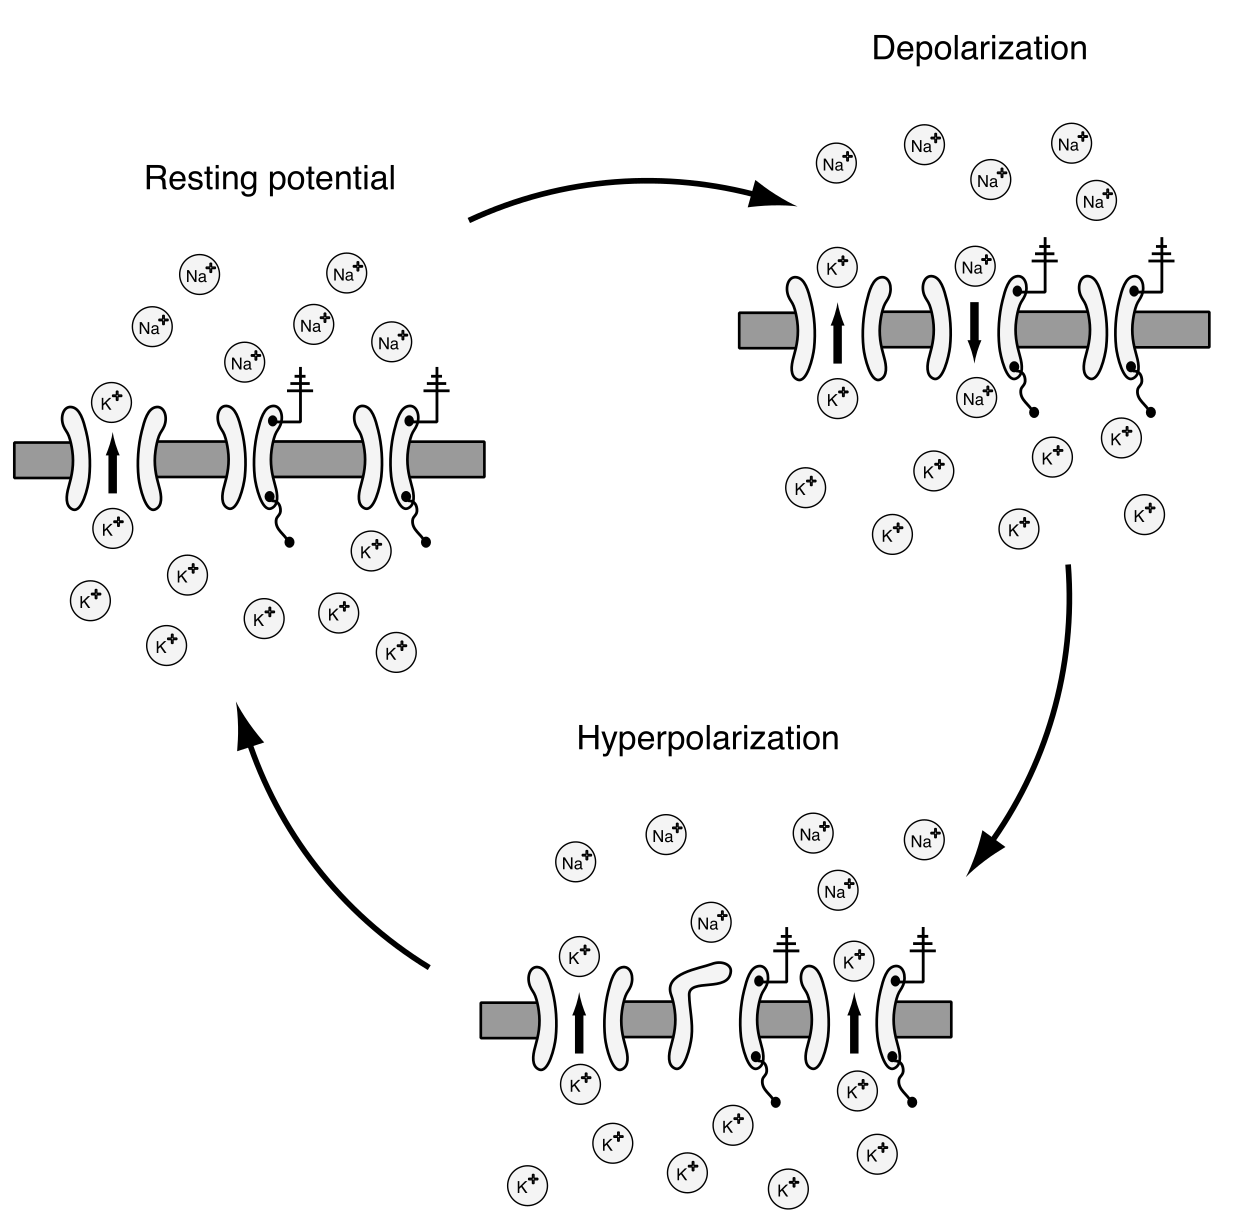
\includegraphics[width=0.7\textwidth]{figures/ion_channel}
    \caption[ساختار کانال‌های یونی]{ساختار کانال‌های یونی \cite{trappenberg2022}}
    \label{fig:ion_channels}
\end{figure}

پلاسمای داخل سلول و مایع اطراف سلول، هر دو محلول‌هایی الکترولیت هستند
\cite{graben2008}.
همان‌طور که در
\autoref{fig:ion_channels}
مشاهده می‌کنید، غلظت یون‌ها در مایع درون سلول با غلظت آن‌ها در مایع اطراف سلول متفاوت است.
این تفاوت غلظت، پتانسیلی الکتریکی ایجاد می‌کند که نقشی مهم در دینامیک نورون دارد
\cite{gerstner2002}.
محیط خارج سلول دارای غلظت بالاتری از یون‌های سدیم
(\ce{Na+})
و کلراید
(\ce{Cl-})
و کلسیم
(\ce{Ca^2+})
است، در حالی که محیط داخل سلول دارای غلظت بالاتری از یون پتاسیم
(\ce{K+})
و مولکول‌های دارای بار منفی
(\ce{A-})
است.
در حالت کلی، غلظت یون‌های منفی در داخل نورون بیشتر است
\cite{izhikevich2006}.
این تفاوت غلظت یون‌ها در داخل و خارج نورون باعث پخش یون‌ها از طریق کانال‌های یونی موجود در سطح غشاء می‌شود.
پمپ‌های یونی در غشای سلولی مسئول حفظ این تفاوت غلظت هستند
\cite{dayan2001}.

بارهای منفی اضافی در درون نورون، که متحرک نیز هستند، یکدیگر را دفع کرده و در سطح داخلی غشای سلولی تجمع می‌کنند.
چگالی برابری از یون‌های مثبت نیز به دلیل نیروهای الکترواستاتیکی، جذب سطح بیرونی غشاء می‌شوند.
این تجمع یون‌ها در دو سمت غشای سلولی یک اختلاف پتانسیل ایجاد می‌کند که به آن پتانسیل غشاء\LTRfootnote{Membrane potential} می‌گویند.
طبق قرارداد، پتانسیل مایع خارج از نورون صفر در نظر گرفته می‌شود
\cite{dayan2001}.
بنابراین، در حالت استراحت، پتانسیل درون غشای سلولی یک نورون حدود ۶۵- میلی‌ولت است
\cite{gerstner2002}.
این پتانسیل توسط معادله نرنست\LTRfootnote{Nernst equation} توصیف می‌شود که کار لازم برای جبران گرادیان انتشار یون‌ها را به لگاریتم نسبت غلظت‌ها، دمای مطلق و برخی پارامترهای خاص سیستم مرتبط می‌کند
\cite{feiner1994}.
این پتانسیل، نقطه تعادلی است که در آن جریان یون‌های ورودی به سلول با جریان یون‌های خروجی از سلول مطابقت دارد.

پتانسیل منفی غشاء، یون‌های مثبت را به داخل نورون جذب و یون‌های منفی را دفع می‌کند.
جریانی از یون‌ها که از طریق تمام کانال‌های یونی از غشاء عبور می‌کنند، جریان غشایی نورون نامیده می‌شود.
این جریان با جمع کردن جریان‌های مربوط به انواع مختلف کانال‌های یونی، از جمله کانال‌های وابسته به پتانسیل و کانال‌های سیناپسی محاسبه می‌شود
\cite{dayan2001}.

هنگامی که جریان یون‌های مثبت به داخل یا جریان یون‌های منفی به خارج از نورون به اندازه‌ای افزایش یابد که پتانسیل غشای نورون از یک حد آستانه مشخص فراتر ببرد، یک فرآیند بازخورد مثبت آغاز می‌شود.
این فرآیند بازخورد مثبت منجر به ایجاد یک پتانسیل عمل می‌شود.
این پتانسیل عمل ایجاد شده، افت‌وخیزهایی ناگهانی و گذرا در پتانسیل غشای سلولی ایجاد می‌کند که در حدود ۱ تا ۲ میلی‌ثانیه طول می‌کشد و در شرایط عادی می‌تواند در محدوده ۹۰- تا ۵۰+ میلی‌ولت تغییر کند.
مقدار پتانسیل غشاء به اندازه‌ای کوچک است که به نورون اجازه می‌دهد از انرژی حرارتی برای انتقال یون‌ها استفاده کند، اما در عین حال به اندازه‌ای بزرگ است که به افت‌وخیزهای دمایی اجازه نمی‌دهد توانایی نورون را در تولید سیگنال‌های الکتریکی مختل کند
\cite{dayan2001}.

پتانسیل عمل واحد اساسی انتقال سیگنال در نورون‌هاست.
اگرچه تمامی پتانسیل‌های عمل یک نورون مشخص شبیه به هم هستند و شکل آن‌ها اطلاعات خاصی را حمل نمی‌کند اما تعداد و زمان‌بندی این پتانسیل‌های عمل است که نقشی اساسی و مهم در انتقال اطلاعات دارند.
معمولاً پتانسیل‌های عمل به خوبی از هم جدا می‌شوند و به دلیل وجود دوره بازیابی\LTRfootnote{ًRefactory period} مطلق، تولید پتانسیل عمل دوم بلافاصله پس از پتانسیل عمل اول غیرممکن است.
حتی با وجود ورودی‌های بسیار قوی، ایجاد پتانسیل عمل دوم در طول یا بلافاصله پس از اولین پتانسیل عمل غیرممکن خواهد بود
\cite{gerstner2002}.

پتانسیل‌های عمل از اهمیت بالایی برخوردارند زیرا تنها شکلی از نوسان‌های پتانسیل غشای سلولی هستند که قادر به انتشار در فاصله‌های طولانی هستند.
این توانایی انتشار سریع و مؤثر، نقش کلیدی در انتقال اطلاعات عصبی ایفا می‌کند.
پتانسیل‌های عمل به طور فعال در طول آکسون بازتولید می‌شوند و می‌توانند به سرعت در فاصله‌های زیاد بدون تضعیف حرکت کنند
\cite{dayan2001}.

کانال‌های یونی وابسته به پتانسیل نقش حیاتی در تولید و انتقال پتانسیل‌های عمل در نورون ایفا می‌کنند.
این کانال‌ها به عنوان تابعی از پتانسیل غشای سلولی عمل می‌کنند و باز و بسته شدن آن‌ها به تغییرات پتانسیل غشاء بستگی دارد.
برای تولید پتانسیل عمل، حداقل دو نوع کانال یونی وابسته به پتانسیل (کانال‌های سدیم و پتاسیم) و یک نوع کانال یونی دیگر نیاز است.

در مرحله ابتدایی از فرآیند پتانسیل عمل، وقتی نورون به اندازه‌ی کافی دیپولاریزه (پتانسیل غشاء مثبت‌تر از پتانسیل استراحت) می‌شود، کانال‌های سدیم
(\ce{Na+})
وابسته به پتانسیل باز می‌شوند.
به دلیل پتانسیل منفی داخل سلول و غلظت کمتر یون‌های سدیم
(\ce{Na+})
در درون سلول نسبت به بیرون، یون‌های سدیم به درون سلول هجوم می‌آورند.
این جریان ورودی از یون‌های سدیم
(\ce{Na+})
باعث افزایش سریع پتانسیل غشاء تا نزدیکی پتانسیل تعادلی سدیم که در حدود ۶۵+ میلی‌ولت است، می‌شود.
این تغییر غلظت یون‌های سدیم، فاز افزایشی پتانسیل عمل را شکل می‌دهد.

بعد از تقریباً ۱ میلی‌ثانیه، کانال‌های سدیم غیرفعال می‌شوند.
این غیرفعال شدن به دلیل مسدود شدن کانال‌های یونی توسط بخشی از پروتئین‌های سازنده آن کانال‌ها رخ می‌دهد.
هم‌زمان با این غیرفعال شدن، کانال‌های پتاسیم
(\ce{K+})
وابسته به پتانسیل باز می‌شوند.
خروج یون‌های پتاسیم از سلول، پتانسیل غشاء را به سمت پتانسیل تعادلی پتاسیم که نزدیک به ۸۰- میلی‌ولت است، کاهش می‌دهد.
این اتفاق باعث هایپرپولاریزه (پتانسیل غشاء منفی‌تر از پتانسیل استراحت) شدن نورون می‌شود.
این هایپرپولاریزه شدن، منجر به بسته شدن کانال‌های پتاسیم و غیرفعال شدن کانال‌های سدیم می‌شود که در نهایت به بازگشت پتانسیل غشاء به حالت استراحت،
\( V_{\text{rest}} \)،
می‌انجامد
\cite{trappenberg2022}.

تولید مکرر پتانسیل عمل منجر به جریان مکرر یون‌های پتاسیم
(\ce{K+})
و سدیم
(\ce{Na+})
به درون و بیرون نورون می‌شود.
با تکرار این فرآیند، غلظت پتاسیم در درون سلول کاهش یافته و غلظت سدیم افزایش می‌یابد.
این روند، در نهایت می‌تواند منجر به عدم تولید پتانسیل عمل شود.
برای جلوگیری از این وضعیت، وجود پمپ‌های یونی ضروری است.
این پمپ‌ها، یون‌های خاصی را برخلاف گرادیان غلظت آن‌ها، بین درون و بیرون غشای نورون منتقل می‌کنند.
این فرآیند، نیاز به انرژی زیادی دارد.
تخمین زده می‌شود که پمپ‌های یونی حدود ۷۰ درصد از کل مصرف متابولیک نورون‌ها و حدود ۱۵ درصد از کل انرژی مصرفی بدن انسان را تشکیل می‌دهند، در حالی که مغز تقریباً یک پنجم کل انرژی بدن را مصرف می‌کند
\cite{trappenberg2022}.

به طور کلی، تمام متغیرهایی که دینامیک نورون را توصیف می‌کنند، با توجه به عملکرد و مقیاس زمانی آن‌ها، می‌توان به چهار دسته تقسیم کرد:
۱- پتانسیل غشاء.
۲- متغیرهای تحریکی که مسئول ایجاد پتانسیل عمل هستند.
۳- متغیرهای بازیابی که مسئول کاهش پتانسیل عمل هستند.
۴- متغیرهای انطباقی که در طول پتانسیل عمل طولانی مدت ایجاد می‌شوند و می‌توانند بر تحریک‌پذیری تأثیر بگذارند
\cite{izhikevich2006}.

\subsubsection{پتانسیل نرنست}
در نظریه ترمودینامیک و فیزیک آماری، احتمال اینکه یک مولکول حالت انرژی
\( E \)
را بگیرد، متناسب با توزیع ماکسول-بولتزمن است، یعنی
\( p(E) \propto \exp \left( -E / kT \right) \)،
که در آن
\( k \)
ثابت بولتزمن و
\( T \)
دماست.
اگر یون‌های مثبت با بار
\( q \)
را در یک میدان الکتریکی ساکن قرار دهیم، انرژی آن‌ها در مکان
\( x \)
برابر است با
\( E(x) = q V(x) \)
که در آن
\( V(x) \)
پتانسیل در مکان
\( x \)
است.
بنابراین، احتمال یافتن یک یون در ناحیه‌ای اطراف
\( x \)
با
\( \exp \left( -q V(x) / kT \right) \)
متناسب است.
از آنجایی که تعداد یون‌ها بسیار زیاد است، می‌توان این احتمال را به عنوان چگالی یون‌ها در نظر گرفت.
بنابراین، برای یون‌های با بار مثبت، چگالی یون‌ها در نواحی با پتانسیل کمتر، بیشتر است.

چگالی یون‌ها در نقطه
\( x \)
را با
\( n(x) \)
نشان می‌دهیم.
نسبت چگالی در مکان
\( x_1 \)
و چگالی در مکان
\( x_2 \)
به صورت زیر است:
\begin{equation} \label{eq:density_ratio}
    \frac{n(x_1)}{n(x_2)} = \exp \left( -\frac{q V(x_1) - q V(x_2)}{kT} \right).
\end{equation}
این معادله نشان می‌دهد که تفاوت در پتانسیل الکتریکی،
\( \Delta V = V(x_1) - V(x_2) \)،
منجر به تفاوت در چگالی یون‌ها می‌شود.
از آنجایی که این معادله در حالت تعادل برقرار است، عکس آن نیز صادق است، یعنی تفاوت در چگالی یون‌ها باعث ایجاد اختلاف پتانسیل الکتریکی می‌شود.

با حل
\autoref{eq:density_ratio}
برای دو ناحیه از یون‌ها با غلظت‌های
\( n_1 \) و \( n_2 \)،
به این نتیجه می‌رسیم که در حالت تعادل، اختلاف غلظت، اختلاف پتانسیلی برابر با مقدار زیر ایجاد می‌کند:
\begin{equation}
    \Delta V = \frac{kT}{q} \ln \frac{n_2}{n_1}.
\end{equation}
این اختلاف پتانسیل را با نام پتانسیل نرنست می‌شناسیم
\cite{hille2001}.

\section{مدل ادغام و آتش}
مدل پایه ادغام و آتش\LTRfootnote{Integrate-and-fire model} که توسط لوئیز لاپیک\LTRfootnote{Louis Lapicque} در سال ۱۹۰۷ پیشنهاد شد، از اولین مدل‌های ریاضی برای توصیف رفتار نورون‌هاست.
این مدل حتی پیش از شناخت کامل مکانیسم‌هایی که پتانسیل عمل را ایجاد می‌کنند، معرفی شده است
\cite{burkitt2006,brunel2007}.
با وجود سادگی و قدمت، این مدل همچنان یک توصیف بسیار مفید از فعالیت‌های نورونی ارائه می‌دهد.

در ساده‌ترین نسخه از این مدل، تمام رسانایی‌های فعال غشاء، از جمله ورودی‌های سیناپسی، نادیده گرفته می‌شوند.
در این حالت، کل رسانایی غشاء به صورت یک عبارت نشتی مدل‌سازی می‌شود:
\begin{equation} \label{eq:leaky_current}
    I_{m} = g_{L} (V - E_{L})
\end{equation}
که در آن
\( I_{m} \)
جریان عبوری از غشاء،
\( g_{L} \)
رسانایی نشتی غشاء و
\( E_{L} \)
پتانسیل نشتی است.
این نسخه از مدل ادغام و آتش به عنوان مدل ادغام و آتش نشتی\LTRfootnote{Leaky integrate-and-fire model} شناخته می‌شود
\cite{dayan2001}.

در این مدل، جریان عبوری از مجموعه‌ای از کانال‌های یونی با نوع
\( i \)
و پتانسیل معکوس
\( E_{i} \)
زمانی متوقف می‌شود که پتانسیل غشاء
\( V \)
برابر با
\( E_{i} \)
شود.
اختلاف
\( V - E_{i} \)
به عنوان نیروی محرکه\LTRfootnote{Driving force} شناخته می‌شود.
جریان غشاء برای کانال‌های نوع
\( i \)
به صورت
\( g_{i} (V - E_{i}) \)
بیان می‌شود
که در آن
\( g_{i} \)
رسانایی غشاء برای کانال نوع
\( i \)
است.
با جمع جریان‌های ناشی از انواع مختلف کانال‌ها، جریان کل غشاء به دست می‌آید
\cite{dayan2001}:
\begin{equation} \label{eq:channel_current}
    I_{m} = \sum_{i} g_{i} (V - E_{i}).
\end{equation}

عمده پیچیدگی و غنای دینامیکی نورون به دلیل تغییرات رسانایی غشاء در طول زمان است.
با این حال، برخی از عواملی که در جریان کل غشاء نقش دارند، می‌توانند نسبتاً ثابت باشند و تحت عنوان جریان نشتی در نظر گرفته شوند.
این جریان نشتی را می‌توان به شکل زیر نوشت:
\[ \bar{g}_{L} (V - E_{L}) \]
که در آن
\( \bar{g}_{L} \)
رسانایی نشتی غشاء و
\( E_{L} \)
پتانسیل نشتی است.
از آنجایی که این عبارت مجموعی از تمام جریان‌های نشتی است، پتانسیل
\( E_{L} \)
معمولاً با پتانسیل تعادل هیچ یون خاصی برابر نیست.
این پتانسیل اغلب به عنوان یک پارامتر آزاد در معادلات نگه داشته می‌شود و به گونه‌ای تنظیم می‌شود که پتانسیل استراحت مدل نورونی با سلول مدل‌سازی شده مطابقت داشته باشد.
به طور مشابه،
\( g_{L} \)
نیز به گونه‌ای تنظیم می‌شود که با رسانایی غشاء در حالت استراحت مطابقت داشته باشد.

همان‌طور که در قبل گفته شد، می‌توان غشاء نورون را به شکل یک خازن در نظر گرفت و مجموع جریان‌هایی که به نورون وارد یا از آن خارج می‌شوند را به شکل زیر
\( C_{m} dV / dt \)
نوشت،
که در آن
\( C_{m} \)
ظرفیت کل نورون و
\( V \)
پتانسیل غشاء است.
با کنار هم قرار دادن جریان‌هایی که در بالا معرفی شد، معادله‌ی پایه برای مدل‌های یک بعدی نورون به دست می‌آید:
\begin{equation} \label{eq:membrane_current}
    C_{m} \frac{dV}{dt} = -I_{m} + I.
\end{equation}
در اینجا
\( I \)
جریان ورودی به نورون است.
ساختار مدلی که در
\autoref{eq:membrane_current}
معرفی شد، مشابه یک مدار الکتریکی است که به آن مدار معادل گفته می‌شود.
همان‌طور که در
\autoref{fig:lif_circuit}
مشاهده می‌کنید، این مدار معادل از یک خازن و مجموعه‌ای از مقاومت‌های متغیر و غیرمتغیر تشکیل شده است
\cite{dayan2001}.

\begin{figure}[!ht]
    \centering
    \begin{circuitikz}
        \draw (1.5,4) to[short, i=\( I \)] (1.5,3);
        \draw (0,0) to[C=\( C_{m} \)] (0,3) -- (3,3) to[R=\( g_{L} \)] (3,1) to[battery1, l=\( E_{L} \)] (3,0) -- (0,0);
        \draw (1.5,0) node[ground] {};
    \end{circuitikz}
    \caption{مدار معادل مدل ادغام و آتش نشتی}
    \label{fig:lif_circuit}
\end{figure}

هنگامی که پتانسیل غشاء یک نورون به آستانه‌ای در حدود ۵۵- تا ۵۰- میلی‌ولت برسد، نورون به طور معمول یک پتانسیل عمل شلیک می‌کند.
این پتانسیل عمل باعث تغییرات سریع و مشخص در پتانسیل غشاء می‌شود که پس از آن، پتانسیل به مقدار اولیه خود که معمولاً هایپرپولاریزه است، باز می‌گردد.
در مدل ادغام و آتش، زمانی که پتانسیل غشاء نورون به مقدار آستانه
\( V_{\text{th}} \)
می‌رسد، پتانسیل عمل رخ می‌دهد.
پس از ایجاد پتانسیل عمل، پتانسیل غشاء به مقدار بازنشانی
\( V_{\text{reset}} \)
که کمتر از آستانه است، بازگردانده می‌شود
\cite{dayan2001}.

معادله‌ی اساسی که رفتار پتانسیل غشاء را در مدل ادغام و آتش نشتی توصیف می‌کند، از ترکیب معادله‌های
\ref{eq:leaky_current} و \ref{eq:membrane_current}
به دست می‌آید.
این معادله به شکل زیر است
\cite{dayan2001}:
\begin{equation} \label{eq:integrate_fire}
    C_{m} \frac{dV}{dt} = - \bar{g}_{L} (V - E_{L}) + I.
\end{equation}
در اینجا
\( C_{m} \)
ظرفیت غشاء،
\( g_{L} \)
رسانایی نشتی،
\( E_{L} \)
پتانسیل نشتی و
\( I \)
جریان ورودی به نورون است.

با توجه به این که مقاومت کل غشاء
\( R_{m} \)
برابر با
\( 1 / g_{L} \)
است، ضرب کردن دو طرف
\autoref{eq:integrate_fire}
در
\( R_{m} \)،
معادله‌ی اساسی مدل ادغام و آتش را به شکل زیر تغییر می‌دهد \cite{dayan2001}:
\begin{equation} \label{eq:leaky_integrate_fire}
    \tau_{m} \frac{dV}{dt} = E_{L} -V + R_{m} I.
\end{equation}

که در آن
\( \tau_{m} = C_{m} R_{m} \)
ثابت زمانی غشاء نورون است.
این معادله نشان می‌دهد که اگر جریان ورودی
\( I \)
برابر صفر باشد، پتانسیل غشاء به طور نمایی با ثابت زمانی
\( \tau_{m} \)
به
\( V = E_{L} \)
که پتانسیل استراحت نورون است، نزدیک می‌شود.
بنابراین،
\( E_L \)
پتانسیل استراحت نورون در این مدل است.
در
\autoref{fig:lif}
رفتار پتانسیل غشاء برای این مدل نشان داده شده است.

\begin{figure}[!htt]
    \centering
    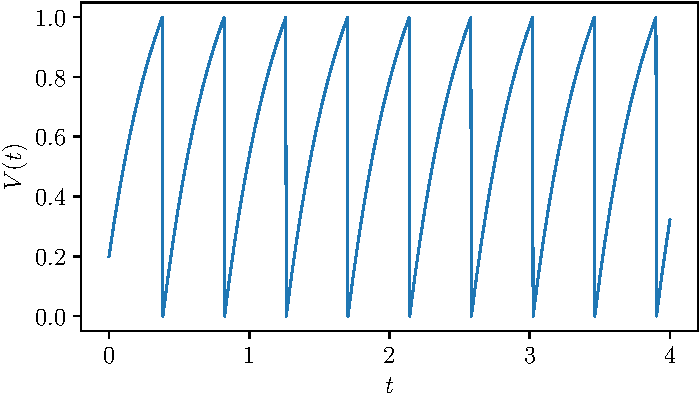
\includegraphics[width=0.8\textwidth]{figures/LIF}
    \caption{رفتار پتانسیل غشاء نسبت به زمان در مدل ادغام و آتش نشتی}
    \label{fig:lif}
\end{figure}

مدل ادغام و آتش که در اینجا توضیح داده شد، بر پایه دو تقریب اساسی است.
توصیف ساده‌ای از پتانسیل عمل و تقریب خطی برای جریان عبوری از کل غشاء
\cite{dayan2001}.

\section{مدل هاجکین-هاکسلی}
این مدل در سال ۱۹۵۲ توسط الن هاجکین\LTRfootnote{Alan Hodgkin} و اندرو هاکسلی\LTRfootnote{Andrew Huxley} معرفی شد
\cite{hodgkin1952,hodgkin1952a,hodgkin1952b,hodgkin1952c,hodgkin1952d}.
آن‌ها با انجام آزمایش‌هایی گسترده بر روی آکسون غول‌پیکر ماهی مرکب و اندازه‌گیری جریان‌های عبوری از غشاء، دینامیک نورون و فرآیند تولید پتانسیل عمل را با استفاده از چهار معادله دیفرانسیل جفت‌شده توصیف کردند
\cite{trappenberg2022}.
در این آزمایش‌ها، آن‌ها سه نوع جریان یونی مختلف شناسایی کردند.
جریان یون‌های سدیم، پتاسیم و یک جریان نشتی که عمدتاً از یون‌های کلراید تشکیل شده بود
\cite{gerstner2002}.

جریان غشاء برای کانال نوع
\( i \)
را می‌توان با استفاده از قانون اهم به صورت زیر بیان کرد:
\begin{equation}
    I_{i} = g_{i} (V - E_{i})
\end{equation}
که در آن،
\( g_{i} \)
رسانایی غشاء و
\( E_{i} \)
پتانسیل استراحت یون
\( i \)
برای هر کانال است
\cite{trappenberg2022}.
جریان کل عبوری از غشای سلولی به شکل زیر بیان می‌شود:
\begin{equation} \label{eq:membrane_current_split}
    C_{m} \frac{dV}{dt} = -\sum_{i} I_{i} + I.
\end{equation}
در اینجا
\( I \)
جریان ورودی به نورون و
\( V \)
پتانسیل غشاء است.

هر کانال یونی را می‌توان با مقاومت یا به طور معادل با رسانایی آن کانال مشخص کرد.
کانال نشتی توسط رسانایی مستقل از پتانسیل
\( g_{L} = 1 / R \)
توصیف می‌شود، در حالی که رسانایی کانال‌های یونی دیگر، وابسته به پتانسیل و زمان هستند.
اگر این کانال‌ها باز باشند، جریان‌هایی را با حداکثر رسانایی
\( g_{\text{Na}} \) یا \( g_{\text{K}} \)
منتقل می‌کنند که به ترتیب حداکثر رسانایی کانال یونی سدیم و پتاسیم هستند.
به طور معمول، بعضی از کانال‌ها بسته هستند و احتمال باز بودن آن کانال‌ها با متغیرهای
\( n \)، \( m \) و \( h \)
توصیف می‌شود.
هاجکین و هاکسلی جریان کل عبوری از این سه کانال یونی را به شکل زیر فرمول‌بندی کردند که مدار معادل آن در
\autoref{fig:hh_circuit}
نشان داده شده است:
\begin{equation} \label{eq:ion_currents}
    \sum_{i} I_{i} = g_{L} (V - E_{L}) + g_{\text{K}} n^{4} (V - E_{\text{K}}) + g_{\text{Na}} m^{3} h (V - E_{\text{Na}}).
\end{equation}
در این معادله، پارامترهای
\( E_{\text{Na}} \)، \( E_{\text{K}} \) و \( E_{L} \)
به ترتیب پتانسیل معکوس برای یون‌های سدیم، پتاسیم و کانال نشتی هستند.

\begin{figure}[!htt]
    \centering
    \begin{circuitikz}
        \draw (3,4) to[short, i=\( I \)] (3,3);
        \draw (0,0) to[C=\( C_{m} \)] (0,3) -- (2,3) to[R=\( g_{L} \)] (2,1) to[battery1, l=\( E_{L} \)] (2,0) -- (0,0);
        \draw (2,3) -- (4,3) to[vR=\( g_{\text{Na}} \), invert] (4,1) to[battery1, l=\( E_{\text{Na}} \)] (4,0) -- (2,0);
        \draw (4,3) -- (6,3) to[vR=\( g_{\text{K}} \), invert] (6,1) to[battery1, l=\( E_{\text{K}} \)] (6,0) -- (4,0);
        \draw (3,0) node[ground] {};
    \end{circuitikz}
    \caption{مدار معادل مدل ادغام و آتش نشتی}
    \label{fig:hh_circuit}
\end{figure}

پتانسیل‌های معکوس و رسانایی‌ها پارامترهایی تجربی هستند.
متغیر
\( n \)
فعال شدن کانال‌های پتاسیم،
\( m \)
فعال شدن کانال‌های سدیم و
\( h \)
غیر فعال شدن کانال‌های سدیم را توصیف می‌کند.
به دلیل وجود توان چهارم
\( n \)، \( n^{4} \)،
در
\autoref{eq:ion_currents}
می‌توان فرض کرد که چهار بار دریچه‌ای\LTRfootnote{Gated charge} متحرک و مستقل در داخل کانال یونی پتاسیم وجود دارد.
به همین ترتیب، برای کانال سدیم به دلیل وجود
\( m^{3} h \)
در معادلات انتظار می‌رود که سه بار دریچه‌ای مستقل و یک زیرواحد بازدارنده وجود داشته باشند
\cite{graben2008}.

سه متغیر
\( n \)، \( m \) و \( h \)
را متغیرهای دریچه‌ای می‌نامند.
این متغیرها توسط معادلات دیفرانسیل زیر توصیف می‌شوند:
\begin{subequations} \label{eq:gated_variables}
    \begin{align}
        \frac{dn}{dt} & = \alpha_n(V) (1 - n) - \beta_n(V)n  \\
        \frac{dm}{dt} & = \alpha_m(V) (1 - m) - \beta_m(V)m  \\
        \frac{dh}{dt} & = \alpha_h(V) (1 - h) - \beta_h(V)h.
    \end{align}
\end{subequations}
در اینجا، تابع‌های تجربی
\( \alpha_{i}(V) \) و \( \beta_{i}(V) \)
نرخ انتقال بین حالت‌های باز و بسته کانال‌ها را توصیف می‌کنند
\cite{izhikevich2006}.
متغیر فعال‌سازی
\( m \)
معمولاً برای پتانسیل‌های غشاء نزدیک به
\( V_{\text{rest}} \)،
نزدیک به صفر است و با افزایش پتانسیل، به مقدار یک می‌رسد.
در مقابل، متغیرهای غیرفعال‌سازی
\( n \) و \( h \)
معمولاً نزدیک به یک هستند و با افزایش پتانسیل به سمت صفر کاهش می‌یابند
\cite{graben2008}.

با ترکیب معادله‌های
\ref{eq:membrane_current_split}، \ref{eq:ion_currents} و \ref{eq:gated_variables}
می‌توان به معادله‌های اصلی مدل هاجکین-هاکسلی دست یافت:
\begin{subequations}
    \begin{align}
        C_m \frac{dV}{dt} & = -g_{L} (V - E_{L}) - g_{\text{K}} n^4 (V - E_{\text{K}}) - g_{\text{Na}} m^3 h (V - E_{\text{Na}}) + I \\
        \frac{dn}{dt}     & = \alpha_n(V) (1 - n) - \beta_n(V)n                                                                      \\
        \frac{dm}{dt}     & = \alpha_m(V) (1 - m) - \beta_m(V)m                                                                      \\
        \frac{dh}{dt}     & = \alpha_h(V) (1 - h) - \beta_h(V)h.
    \end{align}
\end{subequations}

رفتار پتانسیل غشاء و تغییرات متغیرهای دریچه‌ای که از معادلات بالا به دست آمده‌اند، در شکل‌های
\ref{fig:hh} و \ref{fig:hh_gates}
نسبت به زمان نشان داده شده‌اند.

\begin{figure}[!ht]
    \centering
    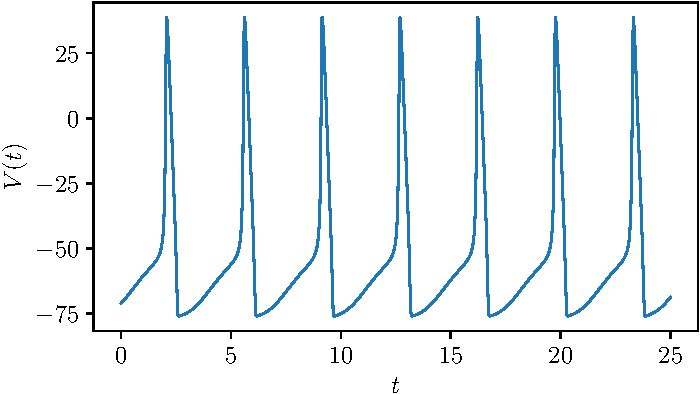
\includegraphics[width=0.8\textwidth]{figures/HH}
    \caption{رفتار پتانسیل غشاء نسبت به زمان در مدل هاجکین-هاکسلی}
    \label{fig:hh}
\end{figure}

\begin{figure}[!ht]
    \centering
    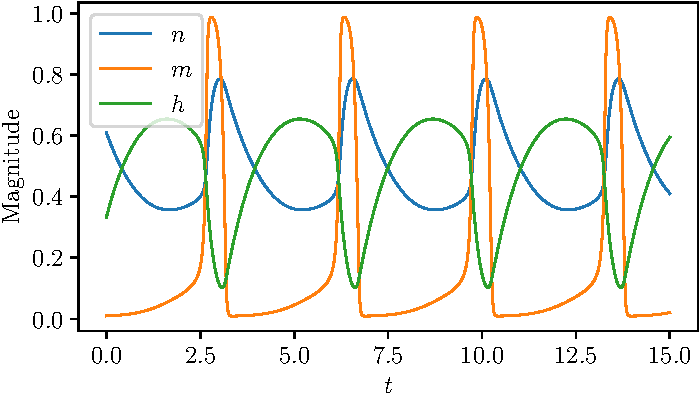
\includegraphics[width=0.8\textwidth]{figures/HH_gates}
    \caption{رفتار متغیرهای دریچه‌ای نسبت به زمان در مدل هاجکین-هاکسلی}
    \label{fig:hh_gates}
\end{figure}

برای درک بهتر رفتار کانال‌های یونی می‌توان متغیرهایی به صورت زیر تعریف کرد:
\[ i_{\infty} = \frac{1}{\alpha_{i} + \beta_{i}}, \qquad \tau_i = \alpha_x i_{\infty}. \]
که در اینجا،
\( i \)
نمایانگر متغیرهای دریچه‌ای
\( n \)، \( m \) و \( h \)
هستند. با استفاده از این دو معادله می‌توان
\autoref{eq:gated_variables}
را به شکل زیر بازنویسی کرد:
\begin{subequations} \label{eq:gated_variables_simplified}
    \begin{align}
        \tau_{n} \frac{dn}{dt} & = n - n_{\infty}(V)  \\
        \tau_{m} \frac{dm}{dt} & = m - m_{\infty}(V)  \\
        \tau_{h} \frac{dh}{dt} & = h - h_{\infty}(V).
    \end{align}
\end{subequations}
در این معادلات، تابع
\( i_{\infty}(V) \)
نشان‌دهنده یک مقدار تعادلی وابسته به پتانسیل غشاء است که به صورت نمایی به ثابت زمانی وابسته به پتانسیل
\( \tau_{i}(V) \)
نزدیک می‌شود.
بررسی رفتار
\( i_{\infty}(V) \)
نسبت به
\( V \)
که در
\autoref{fig:hh_gates_steady}
نشان داده شده است، نشان می‌دهد که رفتار دو تابع از تابع‌های
\autoref{eq:gated_variables_simplified}
شباهت زیادی به هم دارند، در حالی که تابع سوم تا حدودی به صورت معکوس دو تابع دیگر رفتار می‌کند.
این شکل خاص از رفتار متغیرهای دریچه‌ای به ما کمک می‌کند تا در آینده مدل‌هایی ساده شده از پتانسیل عمل را بر اساس این مدل ارائه کنیم
\cite{trappenberg2022}.

\begin{figure}[!ht]
    \centering
    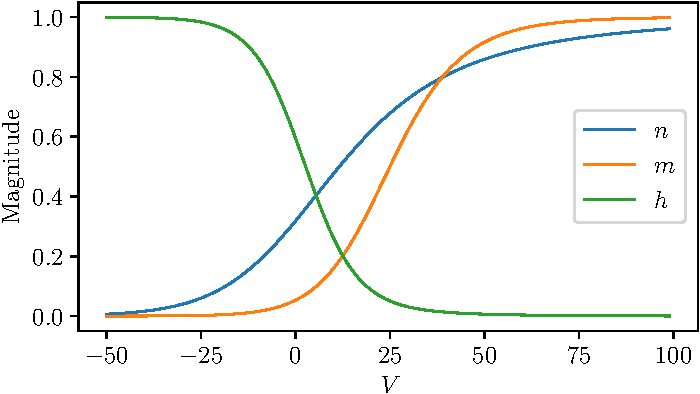
\includegraphics[width=0.8\textwidth]{figures/HH_gates_steady}
    \caption{رفتار حالت تعادلی متغیرهای دریچه‌ای نسبت به پتانسیل غشاء در مدل هاجکین-هاکسلی}
    \label{fig:hh_gates_steady}
\end{figure}

تحلیل رفتار معادلات دیفرانسیل غیرخطی با ابعاد بالا بسیار دشوار است.
در حالی که معادلات دیفرانسیل دو بعدی را می‌توان با استفاده از تحلیل فضای فاز در دو بعد به راحتی مطالعه کرد.
بنابراین، کاهش معادله‌ی چهار بعدی هاجکین-هاکسلی به یک مدل نورونی دو متغیره بسیار مطلوب است
\cite{gerstner2002}.

همان‌طور که در
\autoref{fig:hh_gates}
مشاهده می‌کنید، مقیاس زمانی تغییرات در متغیر دریچه‌ای
\( m \)
بسیار سریع‌تر از متغیرهای
\( n \)، \( h \) و \( V \)
است.
این مشاهده نشان می‌دهد که می‌توان
\( m \)
را به عنوان یک متغیر آنی در نظر گرفت.
در این صورت، متغیر
\( m \)
در معادلات مدل هاجکین-هاکسلی را می‌توان با مقدار حالت پایدار آن یعنی
\( m_{0} \)
جایگزین کرد.
به این تقریب، تقریب شبه حالت پایدار گفته می‌شود
\cite{gerstner2002}.

همچنین، با توجه به
\autoref{fig:hh_gates_steady}،
ثابت‌های زمانی
\( \tau_{n}(V) \) و \( \tau_{h}(V) \)
تقریباً برابر هستند.
علاوه بر این،
\( n(V) \) و \( 1 - h(V) \)
نیز تقریباً رفتاری مشابه دارند.
بنابراین می‌توان دو متغیر
\( n \) و \( 1 - h \)
را با یک متغیر مؤثر
\( w \)
تقریب زد
\cite{gerstner2002}.

\section{مدل فیتزهیو-ناگومو}
در سال ۱۹۶۱ و اندکی پس از معرفی مدل هاجکین-هاکسلی، ریچارد فیتزهیو\LTRfootnote{Richard FitzHugh} مدلی را پیشنهاد کرد که به عنوان تعمیمی از نوسانگر وان در پل\LTRfootnote{Van der Pol oscillator} در نظر گرفته می‌شود
\cite{fitzhugh1961}.
جین‌ایچی ناگومو\LTRfootnote{Jinichi Nagumo} و همکارانش در سال ۱۹۶۲ مدار معادل این مدل را معرفی کردند
\cite{nagumo1962}.
این مدل، نسخه‌ای ساده شده از مدل هاجکین-هاکسلی است
\cite{sherwood2014}.
فیتزهیو و ناگومو احتمالاً اولین کسانی بودند که پیشنهاد کردند می‌توان چهار معادله هاجکین-هاکسلی را به دو معادله کاهش داد
\cite{gerstner2002}.

این مدل شامل دو معادله دیفرانسیل غیرخطی جفت‌شده است.
یکی از این معادلات، تحول سریع پتانسیل غشاء نورونی را توصیف می‌کند، در حالی که معادله دیگر، رفتار کندتر بازیابی و غیرفعال شدن کانال‌های سدیم و پتاسیم را نشان می‌دهد
\cite{sherwood2014}.

معادله‌ی اصلی وان در پل، یک معادله دیفرانسیل خطی مرتبه دوم است:
\begin{equation}
    \frac{d^2 V}{dt^2} + (V^2 - 1) \frac{dV}{dt} + \phi V = 0
\end{equation}
که می‌توان آن را با معرفی متغیر
\( W = -dV /dt + V - V^3 / 3 \)
به دو معادله مرتبه اول تبدیل کرد:
\begin{subequations}
    \begin{align}
        \frac{dV}{dt} & = V - \frac{V^3}{3} - W \\
        \frac{dW}{dt} & = \phi V.
    \end{align}
\end{subequations}

همان‌طور که از معادلات بالا پیداست، برای همه مقادیر
\( \phi \)
بزرگ‌تر از صفر، مبدأ یک نقطه ثابت ناپایدار برای این معادلات است.
فیتزهیو با اضافه کردن دو عبارت خطی به معادلات بالا که باعث جابجایی و پایدار کردن نقطه ثابت شد، مدل خود را تکمیل کرد:
\begin{subequations}
    \begin{align}
        \frac{dV}{dt} & = V - \frac{V^3}{3} - W + I \\
        \frac{dW}{dt} & = \phi(V + a - bW).
    \end{align}
\end{subequations}
در اینجا،
\( V \)
نشان‌دهنده پتانسیل غشاء،
\( W \)
یک متغیر بازیابی و
\( I \)
جریان ورودی به نورون است.
مقدارهای
\( a \)، \( b \) و \( \phi \)
نیز ثابت‌هایی مثبت هستند.
در
\autoref{fig:fhn}
رفتار دو متغیر
\( V \) و \( W \)
برای یک جریان ورودی ثابت را مشاهده می‌کنید.

\begin{figure}[!ht]
    \centering
    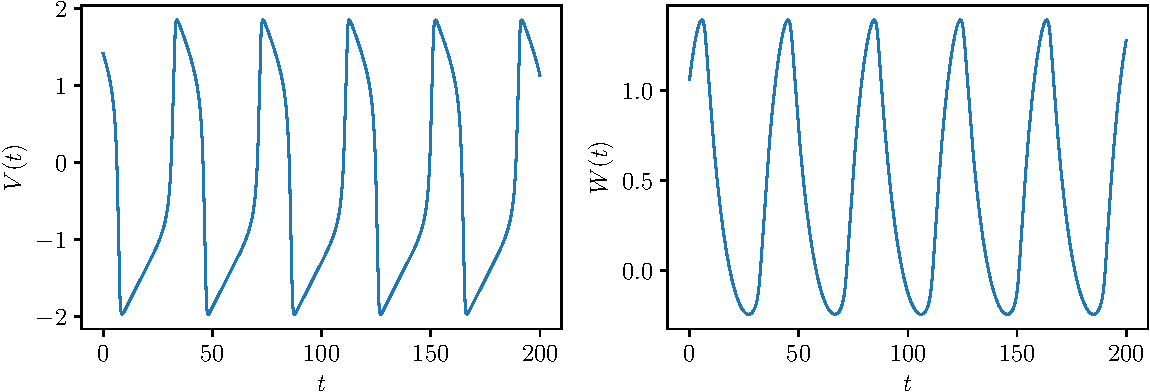
\includegraphics[width=0.95\textwidth]{figures/FHN}
    \caption{رفتار پتانسیل غشاء
        \( V(t) \)
        و متغیر بازیابی
        \( W(t) \)
        در مدل فیتزهیو-ناگومو}
    \label{fig:fhn}
\end{figure}

\section{نگاشت چیالوو}
با توجه به این که ارتباط بین نورون‌ها تنها به پتانسیل‌های عملی که به سیناپس‌ها می‌رسند حساس است، مدل‌سازی این پتانسیل‌های عمل در تحلیل دینامیک یک نورون اهمیت ویژه‌ای دارد.
تاکنون، مدل‌هایی را بررسی کرده‌ایم که با رویکردی مکانیکی یا زیست‌فیزیکی، رفتار دینامیکی پتانسیل غشاء و پتانسیل‌های عمل را مدل‌سازی کرده بودند.
رویکردی دیگر برای مدل‌سازی رفتارهای دینامیکی نورون، رویکرد پدیدارشناختی است.
این رویکرد می‌تواند به توسعه مدل‌هایی از نورون منجر شود که مبتنی بر نگاشت‌ها هستند
\cite{girardi-schappo2013}.

برای دستیابی به مدل‌های عصبی مبتنی بر نگاشت‌ها با ویژگی‌های دینامیکی واقعی، دو مسیر اصلی وجود دارد.
یکی از این مسیرها، استفاده از مدل‌های مشابه هاجکین-هاکسلی است که با معادلات دیفرانسیل غیرخطی جفت‌شده توصیف می‌شوند.
این مدل‌ها که به مدل‌های مبتنی بر رسانایی معروف هستند، خود ساده شده‌ی مجموعه‌ای از معادلات دیفرانسیل جزئی هستند که رفتار غشاء نورون را توصیف می‌کنند.
اگر از این معادلات دیفرانسیل به صورت عددی و با استفاده از روش اویلر با گام زمانی بزرگ انتگرال‌گیری شود، می‌توان به نگاشت‌هایی با ویژگی‌های دینامیکی مشابه سیستم اصلی دست یافت
\cite{ibarz2011,girardi-schappo2013}.

مسیر دیگر در مدل‌سازی پدیدارشناختی می‌تواند از سیستم‌های زمان گسسته آغاز شود.
در این روش، با افزایش پیچیدگی‌های دینامیکی، مدل‌هایی تولید می‌شوند که دینامیک نورون را بازتولید می‌کنند.
این رویکرد زمانی اهمیت پیدا می‌کند که تمرکز ما بر مطالعه ساختار بیوفیزیکی نورون نباشد و مدل‌سازی زیست‌فیزیکی جزئیات بی‌اهمیت تلقی شود، به ویژه در مواردی که تمرکز بر مطالعه رفتاری خاص در یک شبکه نورونی باشد
\cite{ibarz2011,girardi-schappo2013}.

از دیدگاه سیستم‌های دینامیکی، خواص زیر را می‌توان به یک نورون نسبت داد \cite{chialvo1995}:
\begin{enumerate}
    \item در عدم حضور اختلال خارجی، سیستم دارای یک نقطه تعادل جاذب است.
    \item فضای فاز به دو ناحیه‌ی زیر آستانه و فرا آستانه تقسیم می‌شود.
          پس از یک اختلال آنی کوچک که سیستم را از حالت استراحت کمی دور کرده اما آن را در ناحیه زیر آستانه نگه می‌دارد، سیستم به سرعت به حالت تعادل برمی‌گردد.
          در مقابل، یک اختلال به اندازه‌ی کافی بزرگ که سیستم را به ناحیه فرا آستانه می‌برد، باعث ایجاد یک گشت و گذار و تغییرات بزرگ در متغیرهای سیستم می‌شود و تا زمانی که سیستم دوباره به حالت استراحت برگردد، ادامه می‌یابد.
          این پاسخ به اختلال، پتانسیل عمل نامیده می‌شود.
    \item در مدت زمان پتانسیل عمل و برای مدت زمانی مشخص بعد از آن، سیستم ممکن است به اختلال خارجی واکنش مشابه‌ای نشان ندهد.
          در فازهای اولیه پتانسیل عمل که به دوره استراحت معروف است، آستانه ممکن است از حالت استراحت دور شده و حتی به شکل گذرا ناپدید شود.
          بنابراین، حداقل دامنه اختلال‌های اعمالی در دوره استراحت که قادر است متغیرهای حالت را به ناحیه فرا آستانه ببرد، تابعی از زمان است.
    \item تحت یک بایاس ورودی، سیستم‌های برانگیخته ممکن است نوسان‌های دوره‌ای از خود نشان دهند.
          این نوسان‌ها در بعضی از سیستم‌ها و برای برخی مقدار پارامترها ممکن است به حالت آشوبناک دوشاخه شود.
\end{enumerate}

دانته چیالوو\LTRfootnote{Dante R. Chialvo} در سال ۱۹۹۵ با استفاده از چهار خاصیت بالا، نگاشت زیر را به عنوان مدلی برای یک نورون معرفی کرد
\cite{chialvo1995}:
\begin{subequations} \label{eq:chialvo_map}
    \begin{align}
        x_{n+1} & = x_{n}^{2} \exp(y_{n} - x_{n}) + k \\
        y_{n+1} & = a y_{n} - b x_{n} + c.
    \end{align}
\end{subequations}

در اینجا
\( x \)
متغیر فعال‌سازی\LTRfootnote{Activation}
و پتانسیل غشای نورون است.
\( y \)
متغیر شبه بازیابی\LTRfootnote{Recovery-like}
و زیروند
\( n \)
نشان‌دهنده گام زمانی متناسب با تحول زمان گسسته سیستم است.
چهار پارامتر این نگاشت به شرح زیر توصیف می‌شوند:
پارامتر
\( k \)
را می‌توان به عنوان یک بایاس ثابت یا یک اختلال افزاینده وابسته به زمان یا یک جریان ورودی خارجی در نظر گرفت.
پارامتر
\( a \)
ثابت زمانی بازیابی است
(\( a < 1 \)).
پارامتر
\( b \)
وابستگی فرایند بازیابی به فعال‌سازی را مشخص می‌کند
(\( b < 1 \)).
پارامتر
\( c \)
نیز یک انحراف\LTRfootnote{Offset} است.

اگرچه برخی ممکن است مدل‌های مبتنی بر نگاشت را از دیدگاه زیستی بسیار ساده بدانند، اما این مدل‌ها گاهی ارتباط زیستی رضایت‌بخشی دارند.
یکی از مزایای مهم این مدل‌ها، قابل قبول بودن استفاده از آن‌ها در سیستم‌های بزرگ‌تر از نظر محاسباتی است.
علاوه بر این، به دلیل پیچیدگی بسیار بالای سیستم‌های نورونی واقعی، مدل‌های مبتنی بر نگاشت به اندازه‌ای ساده هستند که بتوان با آن‌ها کار کرد، اما در عین حال قادرند ویژگی‌های اصلی و مرتبط نورون‌ها را به خوبی به تصویر بکشند
\cite{pilarczyk2023}.

نقاط ثابت مدل نگاشت چیالوو
\( x_{f} \)، \( y_{f} \)
از روابط زیر به دست می‌آیند:
\begin{subequations} \label{eq:fixed_points}
    \begin{align}
        x_{f} & = x_{f}^{2} \exp(y_{f} - x_{f}) + k                                \\
        y_{f} & = a y_{f} - b x_{f} + c \implies y_{f} = \frac{c - b x_{f}}{1 - a}
    \end{align}
\end{subequations}

در
\autoref{eq:fixed_points}،
اگر
\( b \ll a \)
شود، مقدار
\( y_{f} \)
برابر با مقداری ثابت می‌شود.
در این حالت،
\autoref{eq:chialvo_map}
به یک نگاشت یک بعدی کاهش می‌یابد:
\begin{subequations} \label{eq:reduced_chialvo_map}
    \begin{align}
        x_{n+1} & = x_{n}^{2} \exp(r - x_{n}) + k \\
        r       & = \frac{c}{1 - a}
    \end{align}
\end{subequations}
در صورتی که
\( k = 0 \)
باشد،
\autoref{eq:reduced_chialvo_map}
رفتاری مشابه نگاشت لجستیک\LTRfootnote{Logistic map} از خود نشان می‌دهد.
همچنین، نقطه
\( (x, y) = (0, c / (1 - a)) \)
همیشه یک نقطه ثابت پایدار و جاذب سیستم است.

برای
\( k \ne 0 \)،
زمانی که
\( a = 0.89 \)، \( b = 0.60 \) و \( c = 0.28 \)
باشد،
\( k \)
را می‌توان به عنوان پارامتر دوشاخگی در نظر گرفت.
برای این انتخاب خاص از مقدار پارامترها و مقدارهای کوچک
\( k \)،
یک نقطه ثابت منحصربه‌فرد وجود دارد که به شکل جهانی جاذب است.
به این مجموعه خاص از پارامترها، ناحیه ساکن-برانگیخته گفته می‌شود.
برای مقدارهای بزرگ‌تر
\( k \)،
دیگر نقطه ثابت منحصربه‌فردی پایدار نیست و ممکن است رفتارهای نوسانی ظاهر شود.
این رفتار، دوشاخه شدن از ناحیه ساکن-برانگیخته به ناحیه نوسانی است.
اگر مقدار
\( k \)
کمی بیشتر شود، رفتار شبه آشوبناک نیز برای برخی از مقدارهای پارامترها مشاهده می‌شود.

در شکل‌های
\ref{fig:xy_excitable} و \ref{fig:xy_chaotic}
می‌توانید رفتار مشاهده‌پذیرهای
\( x \) و \( y \)
و همچنین فضای فاز نگاشت چیالوو را برای مرز ناحیه غیربرانگیخته و برانگیخته با پارامتر‌های
\( a = 0.89 \)، \( b = 0.60 \)، \( c = 0.28 \) و \( k = 0.030 \)
و مرز ناحیه غیربرانگیخته و آشوبناک با پارامتر‌های
\( a = 0.89 \)، \( b = 0.18 \)، \( c = 0.28 \) و \( k = 0.023 \)
مشاهده کنید.
این مقدارها برای پارامترها با بیشینه کردن مقدار خودهمبستگی مشاهده‌پذیر
\( x \)
به دست آمده‌اند
\cite{moraes2023}.

\begin{figure}[!ht]
    \centering
    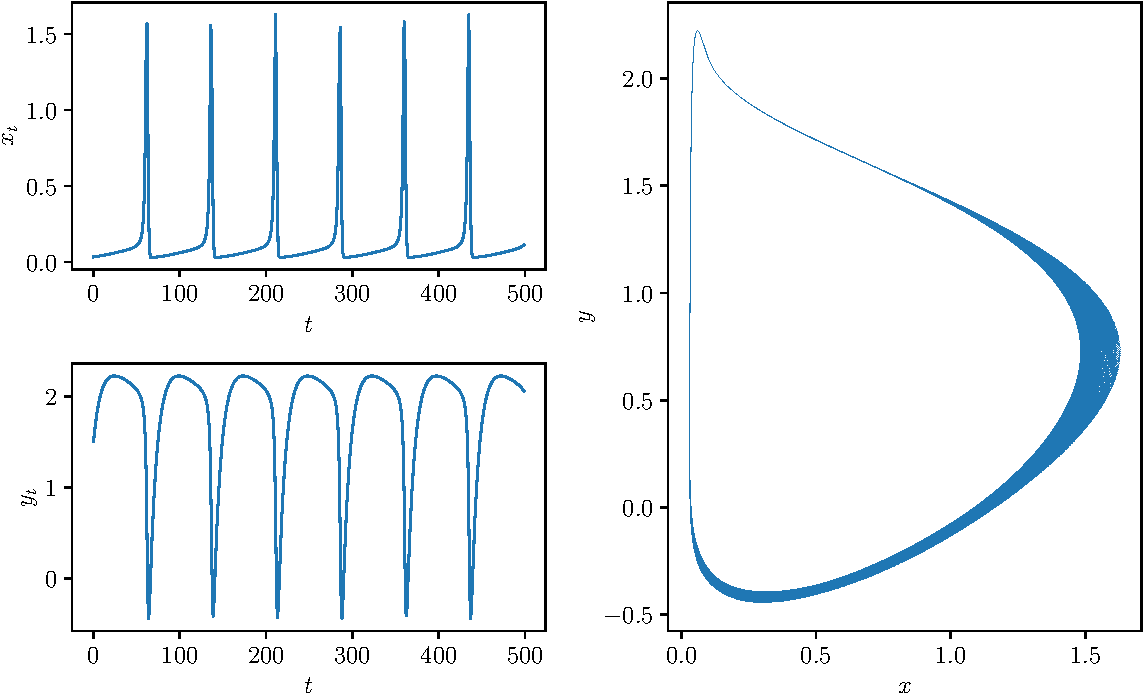
\includegraphics[width=0.9\textwidth]{figures/xy_excitable}
    \caption{
        فضای فاز و رفتار متغیرهای پتانسیل غشاء
        \( x \)
        و بازیابی
        \( y \)
        برای نگاشت چیالوو در ناحیه برانگیخته
    }
    \label{fig:xy_excitable}
\end{figure}

\begin{figure}[!ht]
    \centering
    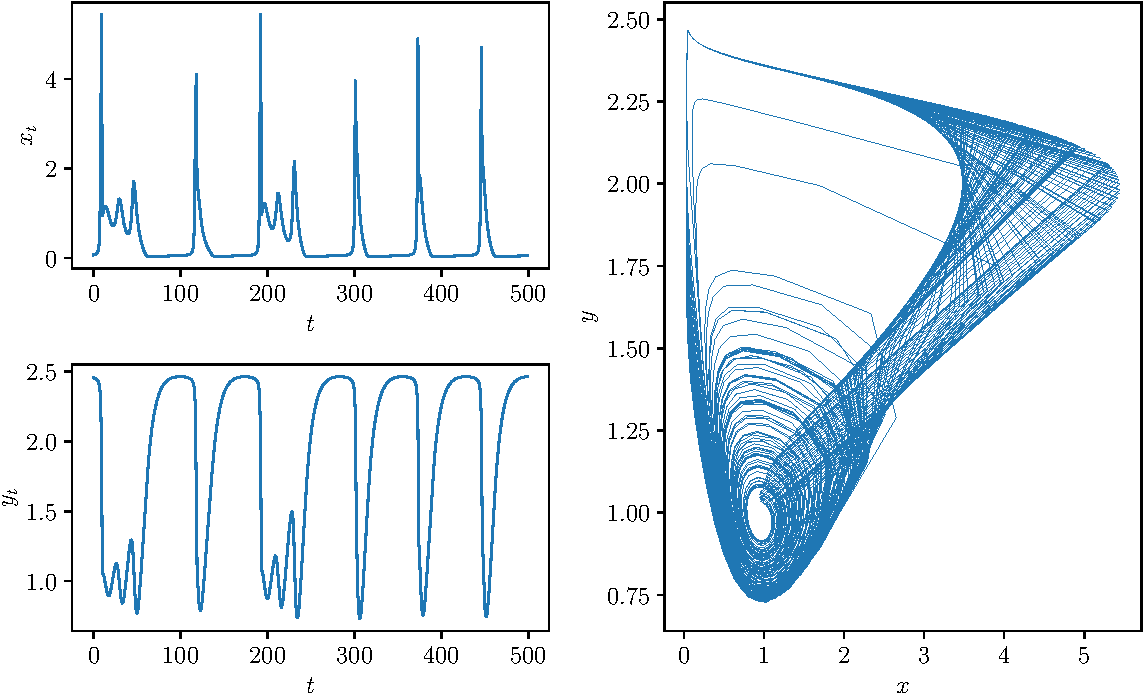
\includegraphics[width=0.9\textwidth]{figures/xy_chaotic}
    \caption{
        فضای فاز و رفتار متغیرهای پتانسیل غشاء
        \( x \)
        و بازیابی
        \( y \)
        برای نگاشت چیالوو در ناحیه آشوبناک
    }
    \label{fig:xy_chaotic}
\end{figure}

برای شناخت بیشتر فضای فاز و رفتار دینامیکی نگاشت چیالوو می‌توانید به \cite{jing2006,courbage2010,wang2018,moraes2023,pilarczyk2023,trujillo2023} مراجعه کنید.
